\documentclass{article}
\usepackage{tikz}
\usetikzlibrary{shapes.geometric}

\begin{document}
\begin{center}
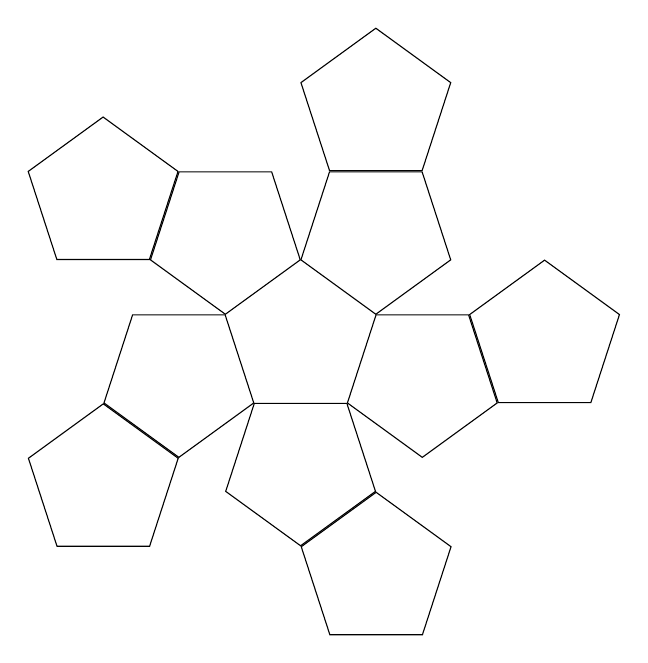
\begin{tikzpicture}[scale=2.2]
  \tikzset{pntgn/.style={regular polygon, regular polygon sides=5,draw,minimum size=2cm,anchor=south}}
  \node(n)[pntgn,draw=none,outer sep=0pt]{};
  \foreach\deg[count=\x] in{36,108,...,324}{\node(m)[pntgn,rotate=\deg,at=(n.side \x)]{};
  \foreach\degg[count=\y] in {36}{\node[pntgn,rotate=\degg+\deg,at=(m.side \y)]{};}}
\end{tikzpicture}
\end{center}
\end{document}
